\chapter{Developing common representations in AI and humans}
\label{chap:common_representations}

In this Chapter we study how human representation and AI representation can be combined, and how brain data can be infused into neural networks.

\section[Using human brain activity to guide machine learning]{\textit{Using human brain activity to guide machine learning}\\ \mandatory{fong2017using}}

This study tries to \textbf{improve ML performance by guiding it with brain activity}, and explore whether such guidance makes the representations themselves more ``human-like". Notice that here the focus is not on performance but on \textbf{representational geometry}. The underlying idea is that, if the human brain is a natural reference point (for representation geometry) and performance, and ANNs are a good algorithm for learning structure, then we can attempt to leverage the ML algorithm with biological information.\\

They consider 7 brain areas (ROIs, \textit{regions of interest}, whose partitioning is defined a-priori). Different brain areas code for different information about the stimulus, but all of them are involved in \textbf{visual processing} (either low, middle, or high level). They use two types of models: CNN and HOG (\textit{histogram of oriented gradients}, an often-used algorithm for generating features that capture the local ``slopeness" of different parts of an image).

Their idea is to train a classifier on brain data to perform binary classification. To do so (to maximize the margin between the decision boundary and the data points), they use a loss derived from the \textbf{Hinge loss} \notet. They define the \textbf{``response strength" from brain fMRI activity data} as the \textbf{distance of an object from the decision boundary} for a given binary classification task.
This produces a per-stimulus activity weight (response strength) for each stimulus. As input to the classifier, each image is encoded as a vector of brain activity values sampled from a given brain area (one of the 7 mentioned before).
From the Hinge loss they define the \textbf{Activation weighted loss} (AWL) as:
\[
\phi (x, z) = max(0, (1-z) \cdot M(x,z)
\]
where $M(x,z) =\begin{cases}
         1+c_x, \text{if } z<1\\
        1 \text{ otherwise}
        \end{cases}$

and $c_x \geq 0$ is an activity weight derived from fMRI data corresponding to $x$ (it is the distance of the object from the classification boundary of the binary classifier trained on brain data).\\
While HL penalizes misclassified examples, \textbf{AWS penalizes misclassified examples on stimuli that are easy for humans to distinguish}.\\

They train a classifier on brain responses (fMRI), then use this prior knowledge to train a new model on non-annotated data. They basically use the learned weights as a starting point. The process consists in the following steps:
\begin{enumerate}
    \item \textbf{Derive per-stimulus ``activity weigths" from fMRI data}:
        \begin{itemize}
        \item collect \textit{per-stimulus} activity vectors: use fMRI to record bold response of subject;
        \item train a classifier on fMRI activity vectors: SVM classifier trained and tested;
        \item activity weights derived from distance boundary: use transformed classification scores.
    \end{itemize}
    \item \textbf{Train (calibrate) 2 image classifiers}:
    \begin{itemize}
        \item Conventional image classifier training: Radial Basis Function SVM classifier;
        \item Margins reweighted by activity data: SVM classifier with activity weighted loss function (note that not all training samples require fMRI weight).
    \end{itemize}
\end{enumerate}

They use images from 5 categories, and the classification problems are based on CNN or HOG features. Information from the higher-level cortical regions is combined in all possible combinations to produce feature sets.

\boxc{\notet Hinge loss}{
The true label is denoted as $t$ ($t=1$ or $t=-1$), while $y$ is the predicted activation for an object by the classifier. $t \cdot y$ is therefore the distance from the boundary. The Hinge loss wants to push this distance so that the margin from the boundary is above 1: 
\[
Loss(y) = max(0, 1-ty)
\]
if $ty <0$ (i.e., incorrect classification) $\Rightarrow 1-ty > 1$;\\
if $0< ty <1$ (correct classification but below the margin) $\Rightarrow 1-ty>0$;\\
if $ty>1$ (correct classification above the margin) $\Rightarrow  1-ty < 0$.\\
This means that the HL is proportional to the distance from the decision boundary, and it \textbf{does not care about magnitude of correct decisions above the margin}.\\

However, in \cite{fong2017using} they use a different formulation:
\[
\phi_h(z) = max(0,1-z)
\]
where $z = y \cdot f(x)$, $y \in N$ is the true label, and $f(x) \in \mathbb{R}$ is the predicted output; thus, $z$ denotes the correctness of a prediction. The HL function assigns a penalty to all misclassified data that is proportional to how erroneous the prediction is.
}

\subsection{Results}
They argue that brain activity compensates for poor feature representation (consider the large difference for HOG in Figure \ref{fig:fong}).

\begin{figure}[!ht]
    \centering
    \captionsetup{width=.8\linewidth}
    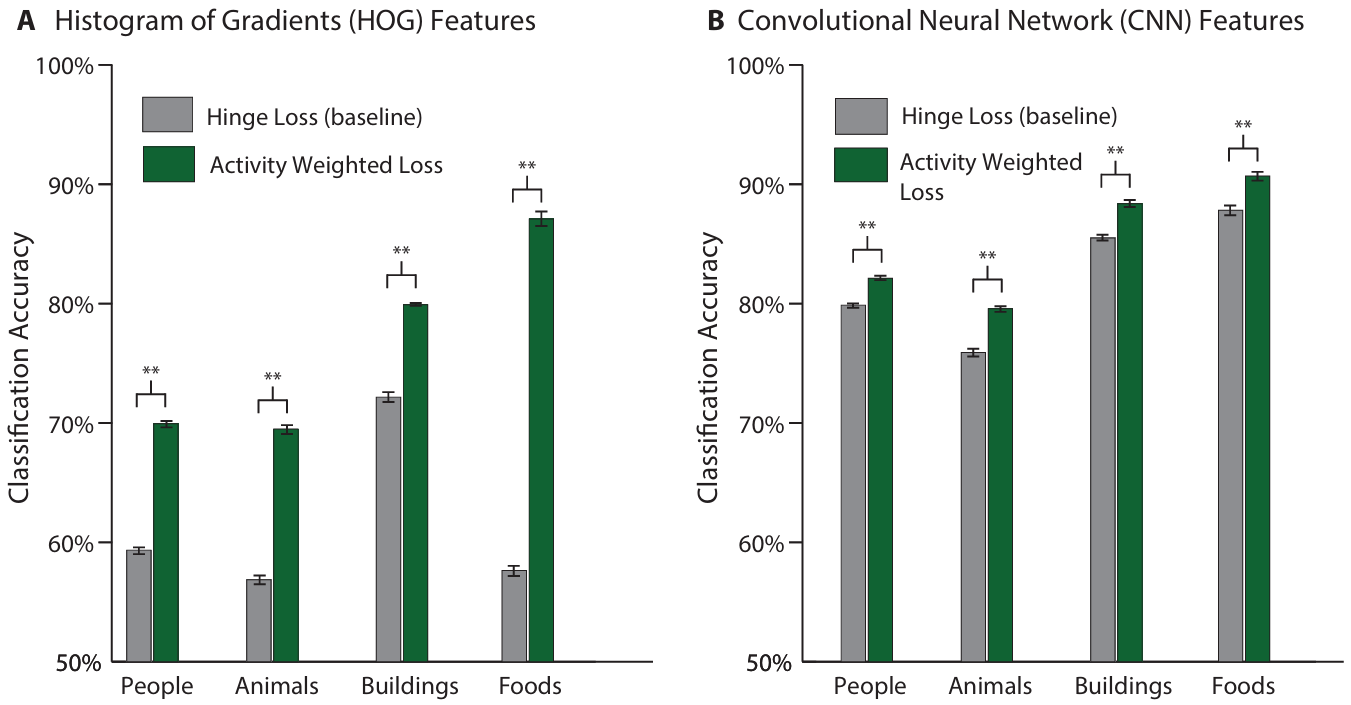
\includegraphics[width=0.65\linewidth]{images/fong.png}
    \caption{Side-by-side comparisons of the mean classification accuracy between models that were trained using either \textbf{(A)} HOG features or \textbf{(B)} CNN features and either a hinge loss (HL) or activity weighted loss (AWL) function.}
    \label{fig:fong}
\end{figure}

They also experiment using information from one brain area only for the loss, observing how this affects classification. Figure \ref{fig:fong_2} shows that certain areas produce significantly better accuracy for the specific categories they are selective for.\\

\begin{figure}[!ht]
    \centering
    \captionsetup{width=.8\linewidth}
    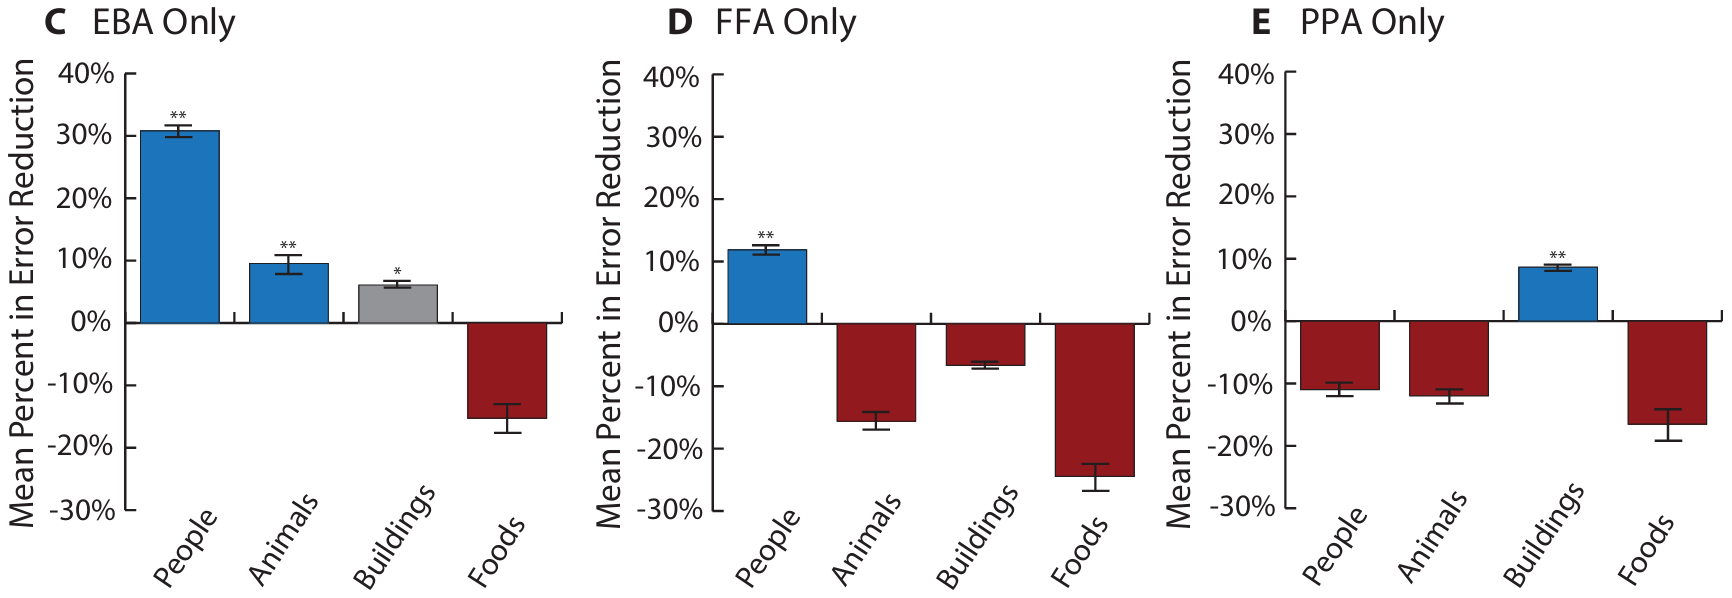
\includegraphics[width=0.7\linewidth]{images/fong_2.png}
    \caption{Mean error reductions gained by switching from HL to AWL loss when using conditioning classifies on brain activity from individual ROIs (i.e., EBA, FFA, or PPA).}
    \label{fig:fong_2}
\end{figure}

In conclusion, \textbf{information measured directly from brain can guide an ML algorithm to make better human-like decisions}.
One can harness measures of the internal representations employed by the brain to guide machine learning.
However, the authors ignore an important question: Are the better results obtained thanks to \textbf{brain} data, or is it just because it is \textbf{more} data? What if we improved the HOG classifier using AWL from CNN classifier (i.e., what if we compute the $C_x$ of the hinge loss from the CNN embeddings?).
The accuracy should be much higher, so we expect the difference when using Activity Weighted Loss to be less significant.

\section[Interpretable semantic vectors from a joint model of brain- and text-based meaning]{\textit{Interpretable Semantic Vectors from a Joint Model of Brain- and Text-Based Meaning}\\ \mandatory{fyshe-etal-2014-interpretable}}

This study is similar to \cite{fong2017using}, but the domain is completely different: human-constraint NLP. They are computational linguists and want to improve word embeddings (they are not really interested in studying the brain).

\subsection{Background}
Vector Space Models (VSMs) represent lexical meaning by assigning each word a point in high dimensional space. The high dimensional space can be any vectorial representation associated with each word. VSMs are typically created using a large text corpora. When this is he case, the VSM represents word semantics as observed in text. In the VSM, the distance between any two words is taken to indicate their semantic similarity (matching, e.g., that observed and rated by speakers). Corpus-based VSMs have been criticized as being noisy or incomplete representations of meaning.\\

When a person is reading or writing, the semantic content of each word necessarily produces patterns of activity over neurons/voxels/sensors. In principle then, \textbf{brain activity could be used instead of corpus data to construct a VSM}. If brain activation data encodes semantics, including brain data in a model of semantics could result in a more effective model. They anticipate that, if it is indeed possible to create word embeddings using brain activations, then the inclusion of this data will only improve a text-based model if brain data contains semantic information not readily available in the corpus.\\

This study tries to:
\begin{itemize}
    \item create a database of human-annotated word semantics and create a brain-informed VSM that better predicts this database,
    \item predict corpus representations of withheld words more accurately by infusing brain data into the learning model,
    \item map semantic concepts onto the brain by jointly learning neural representations.
\end{itemize}

\subsection{Data and method}
The corpus data are compiled from a 16 billion word subset of ClueWeb09 and contain two types of corpus features: \textbf{dependency} (between words) and \textbf{document features}. Dependency statistics were derived by dependency parsing the corpus and compiling co-occurence counts for all dependencies incident on the word. Count thresholding was applied to reduce noise, and positive pointwise mutual-information (PPMI \notet) was applied to the counts. SVD was applied to the document. They started with a word-by-word co-occurence matrix and then get a word-by-feature matrix $X$, after PPMI and SVD.
\osst{They consider just the positive PMI, i.e., words that co-occur more often that if they were independent.}

The brain data comes from fMRI data and MEG data for 18 subjects (9 in each imaging modality). Each read 60 concrete nouns. The 60 words span 12 word categories.\\

They adopt two methods: NNSE and JNNSE.

\subsubsection{Non-Negative Sparse Embedding (NNSE)}
They want to approximate $X$ by matrix factorization, i.e., get two matrices $A$ and $D$ that when multiplied together approximate $X$. $A$ has the same number of rows (words) as $X$, but with a much lower number of latent dimensions (they are trying to compress the feature space), $D$ instead has the same number of columns but less rows. NNSE is therefore defined as follows:
\[
\argmin_{A,D} \sum_{i=1}^w \lVert X_{i,:} - A_{i,:} \times D \rVert^2 + \lambda \lVert A\rVert_1
\]
subject to:
\[
D_{i,:}D_{i,:}^T \leq 1 \quad(\forall \;1 \leq i \leq l)
\]
\[
A_{i,j} \geq 0,\quad 1 \leq i \leq w,\quad 1 \leq j \leq l
\]
The matrix $A$ is the output of the algorithm, i.e., the sparse approximated representation we look for (note the $\lambda \lVert A\rVert_1$ term that induces sparsity).\\

Applying NNSE is important for interpretability: without reducing the number of dimensions, the matrix is likely to have many columns that are correlated. With fewer columns, they can study them as they are not linearly dependent.
The meaning of a word is captured by finding the top-scoring dimensions for the word (i.e., the colums with highest values for the word’s row), and then finding the words that score highest on those dimensions. Each of these dimension, with the set of associated words, captures a meaning of the original word. For example, the word \textit{chair} has the following top-scoring dimensions: 
\begin{enumerate}
    \item chairs, seating, couches;
    \item mattress, futon, mattresses;
    \item supervisor, coordinator, advisor.
\end{enumerate}
These dimensions cover two of the distinct meanings of the word chair (\textit{furniture} and \textit{person of power}).

\subsubsection{Joint Non-Negative Sparse Embedding (JNNSE)}
They extend NNSEs to incorporate an additional source of data for a subset of the words in $X$, and call the approach JNNSEs.
Such algorithm allows to have a ``shared semantic space" (the matrix $A$ is an approximation of both $X$ and $Y$, $Y$ being the $word \times voxel$ matrix), and is defined as follows:
\[
\argmin_{A,D^{(c)},D^{(b)}} \sum_{i=1}^w \lVert X_{i,:} - A_{i,:} \times D^{(c)} \rVert^2 +  \sum_{i=1}^{w'} \lVert Y_{i,:} - A_{i,:} \times D^{(b)} \rVert^2 + \lambda \lVert A\rVert_1
\]
subject to:
\[
D_{i,:}^{(c)}D_{i,:}^{(c)T} \leq 1 \quad(\forall \;1 \leq i \leq l)
\]
\[
D_{i,:}^{(b)}D_{i,:}^{(b)T} \leq 1 \quad(\forall \;1 \leq i \leq l)
\]
\[
A_{i,j} \geq 0,\quad 1 \leq i \leq w,\quad 1 \leq j \leq l
\]
Notice the difference in summation. The first expression goes over all the words in the corpus ($w$), while the second goes over the subset for which we have brain data ($w'$).
$A'$ is the subset of the $A$ matrix that is relevant for reconstructing $Y$ (it is a subset of the rows in X).
Both $X$ and $Y$ can be reconstructed by multiplying $A$ with $D^{(c)}$ and $D^{(b)}$ respectively.\\

JNNSE has many advantages:
\begin{itemize}
    \item Handle partially paired data, compared to Canonical Correlation Analysis or Partial Least Squares that require data about the same observations in both cases;
    \item No need to have a common average brain (can concatenate activation across subjects in the Y matrix, per word), provided we merge different brain imaging experiments adding the specific term to the loss (to learn a different $D^{(b)}$ matrix for each subject).
\end{itemize}

\subsection{Experiments and results}
To check whether the word-by-feature matrix encodes for specific properties, they use a \textbf{probing classifier}: they train the regression model on $A$ and evaluate it on a human-rated-property table. More specifically, they obtain behavioral measure of semantics for 60 words, rated on 218 properties (e.g. \textit{smell}, \textit{emotion}, etc.), and then train the classifier to predict the [$60 \times 218$] human behavior's matrix from the $A$ matrix obtained using NNSE (text only) or JNNSE (brain+text). They experiment with different numbers of latent dimensions $l$: 250, 500 or 1000. For \textbf{evaluating the correlation} of the latent representation ($A$) with behavioral data ($Y$), they do not compare the tables directly, but use in-matrix pairwise (Euclidean) distance instead, i.e., they are somehow checking if the two vector spaces are isomorphic.\\
Figure \ref{fig:jnnse} shows that joint embeddings improve prediction of human similarity space. However, as in \cite{fong2017using}, the higher performance might not be caused by infusing brain data, but just by using a multiple data sources, which allow to remove noise.\\

Another experiment they deal with consists in \textbf{word prediction from brain data}. The matrix $A$ from NNSE or JNNSE is used as outcome variable: they predict it (for left out words) one column at a time. For each lower-dimension, there is a set of values over words ($Y$).
Regression is used to predict the value of that dimension $l$ over the $Y$ words. This is repeated for all $l$ dimensions, which produces a predictive $l$-dimensional vector per word. They train the regression on $A$ (NNSE or JNNSE) consisting of 58 words. They then produce predictive vectors for the 2 left out words and evaluate their similarity to the ground truth of those embeddings in $A$.\\
The results presented in Figure \ref{fig:jnnse_2} show how word prediction from brain data improves when the embedding space itself ($A$) is constrained by brain data.

\begin{figure}[!ht]
    \centering
    \captionsetup{width=.8\linewidth}
    \begin{subfigure}{.49\textwidth}
        \centering
        \captionsetup{width=.8\linewidth}
        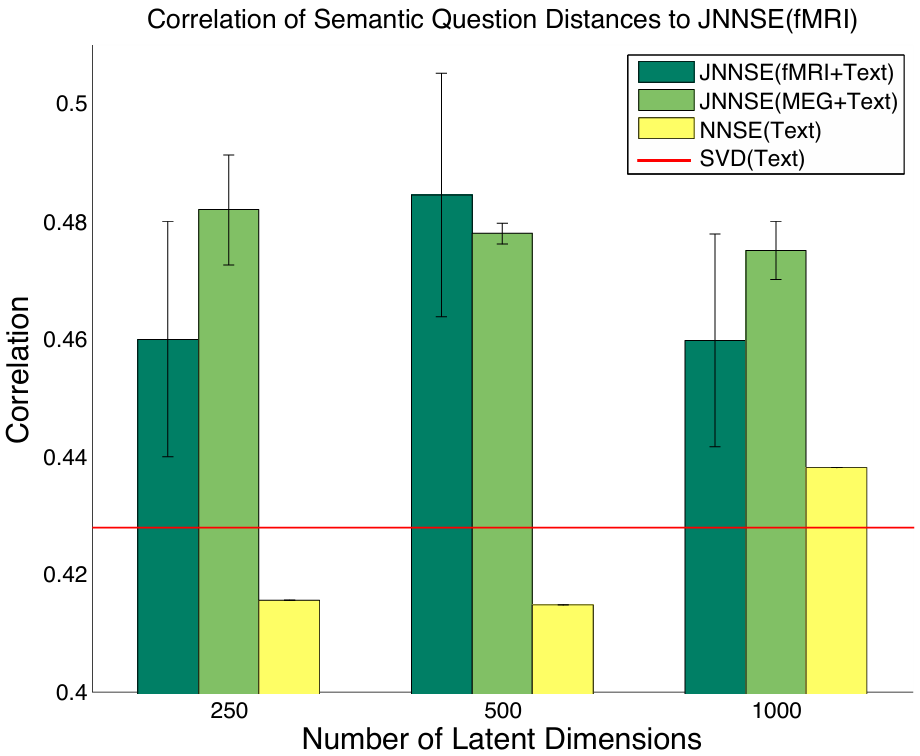
\includegraphics[width=.7\linewidth]{images/jnnse.png}
        \caption{Correlation of NNSE and JNNSE models with the distances in a semantic space constructed from behavioral data.}
        \label{fig:jnnse}
    \end{subfigure}
    \begin{subfigure}{.49\textwidth}
        \centering
        \captionsetup{width=.8\linewidth}
        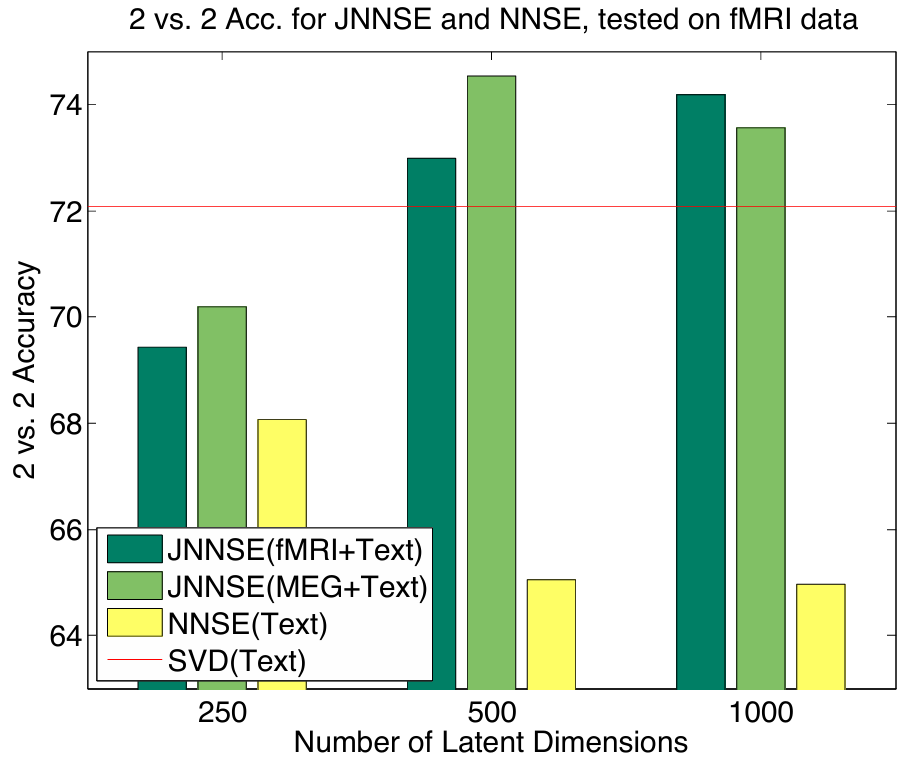
\includegraphics[width=.65\linewidth]{images/jnnse_2.png}
        \caption{Average 2~vs.~2 accuracy for NNSE and JNNSE, tested on fMRI data. Models created with one subject’s fMRI data were not used to compute 2~vs.~2 accuracy for that same subject.}
        \label{fig:jnnse_2}
    \end{subfigure}
    \caption{Comparison between NNSE and JNNSE.}
    \label{fig:jnnse_comp}
\end{figure}

Here they ask: can an accurate latent representation of a word be constructed using only brain activation data? They try to produce $X$-matrix (``raw") entries for words for which there is not enough corpus data required for creation of corpus statistics (i.e., they present rare words to people to get fMRI/MEG data). This experiment practically consists in \textbf{predicting corpus data}. They use JNNSE to obtain $A$-entries for words appearing in $X$ and $Y$ (corpus and brain), but also some words appearing only in $Y$ (brain). Notice that JNNSE allows to have brain activation entries without the corresponding corpus entries.
Then, $D^{(c)}$ in used to recreate the entries for those words.\\
They compute a rank accuracy measure and the mean rank accuracy is as high as 67\% for $l=500$.\\

The last experiment consists in \textbf{mapping semantics onto the brain}. $D^{(b)}$ is a [$l \times v$] matrix (\textit{latent dimensions} $\times$ \textit{voxels}). This allows to obtain a brain map for each dimension $l$ in that matrix. They tweak the importance of the perceptual features ($Y$) by scaling their values (details missing; but we can consider weighting schemes). They plot these dimensions on brain slices. They can find a brain area, link it to the dimension that predicted it, and see which words load strongly on that dimension. This allows to study how different groups (age, culture, etc.) have different representations of language.

\begin{wrapfigure}[12]{r}{0pt}
  \centering
  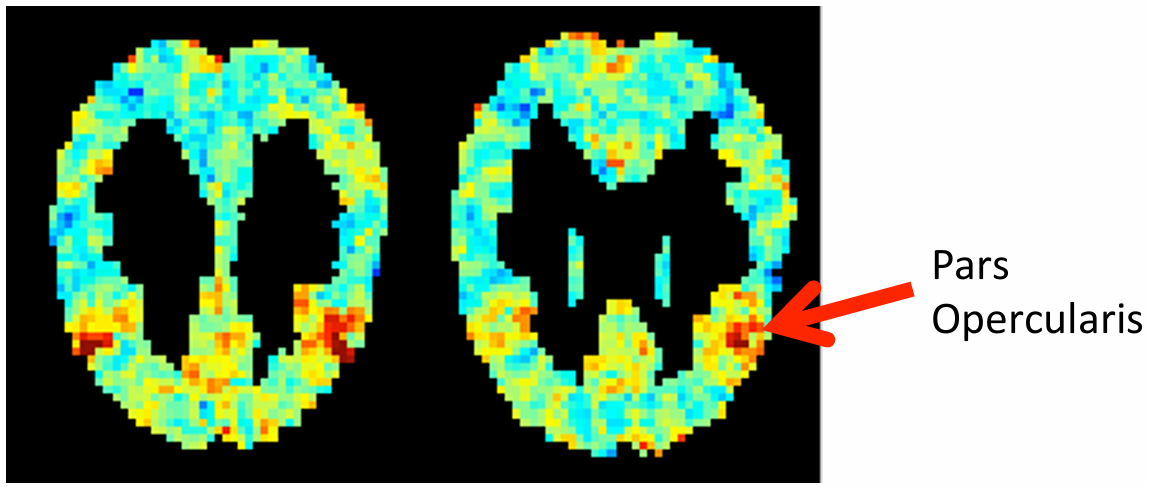
\includegraphics[width=0.4\textwidth]{images/jnnse_4.png}
  \caption{$D^{(b)}$ matrix; dimension with top scoring words \textit{buffet}, \textit{brunch}, \textit{lunch}. Pars opercularis is believed to be part of the gustatory cortex, which responds to food related words.}
  \label{fig:jnnse_4}
\end{wrapfigure}
In Figure \ref{fig:jnnse_4} there is an example (through fMRI slices) of mapping ($D^{(b)}$) from latent semantic space ($A$) to brain space ($Y$) for fMRI and words from three semantic categories.\\

In conclusion, VSMs can be extended or even substituted using brain data. Addition of brain data strongly improves the prediction of human annotations (perhaps can substitute them) and the prediction of latent dimension scores produced in the joint embedding. It is possible to use brain data to synthesize raw corpus data for those words. And finally, solutions of joint embeddings can be mapped onto the brain space.


\section[Decoding brain representations by multimodal learning of neural activity and visual features]{\textit{Decoding Brain Representations by Multimodal Learning of Neural Activity and Visual Features}\\ \mandatory{palazzo2020decoding}}

The idea of this paper we are interested in is: studying attention and saliency on images by infusing brain data into a neural network. In particular, they aim at:
\begin{itemize}
    \item achieving multimodal learning that projects brain data and image data into the same latent space;
    \item using brain activity to guide machine learning tasks (\textbf{visual saliency modeling}).
\end{itemize}

Most prior work in multimodal learning tries to learn a joint embedding space for images and text. Here instead, they try to learn a joint embedding of EEG and images.
The first problem when creating a joint embedding of EEG and images is that the image does not change over time, while the EEG data does. They need an architecture able to encode time.

\subsection{Data and method}
They have EEG data of 6 people watching 40 categories from ImageNet (50 images in each class). The EEG data is at high resolution: 128 channels, 1kHz recording, 0.5sec each image (so that they collect 500 time-points for each image).\\

They use a Siamese network with the triplet loss to maximize the similarity between modalities. EEG ($e$) and visual ($v$) features of the same image ($e_1$, $v_1$) should be mapped to be nearby in image space, whereas EEG features of image 1 and visual features of image 2 ($e_1$, $v_2$) should be pushed apart.
As \textbf{compatibility} (the measure of how much two encodings are similar) between features, they just take the \textbf{dot product of the embeddings}.
Similarity of mismatching EEG/vision should be lower than the matching case.
The loss is defined as follows:
\[
L(e_1, v_1, v_2) = max{0, F(e_1, v_2) - F(e_1, v_1)}
\]
where $F$ is a similarity measure.\\
The triplet loss is positive if the similarity of $e_1$ with $v_2$ (negative item) is greater than its similarity with the positive item ($v_1$).\\

The model receives more than one input at a time (in particular there are two networks, and in total a triplet of inputs is presented). The two networks have the same exact architecture (Figure~\ref{fig:palazzo}). The EEG data are pushed through four 1D-convolutional layers (learning filters at different temporal scales), and these are fed into a recurrent layer. The hidden state of the recurrent layer is fed to a fully connected layer from which embeddings are extracted for the compatibility function.
They don't use directly the embeddings of VGG (or other), but rather put a layer in between (to learn more ``brain related" representations: they train different architectures, whose representations are fine-tuned during the Siamese training.

\begin{figure}[!ht]
    \centering
    \captionsetup{width=.8\linewidth}
    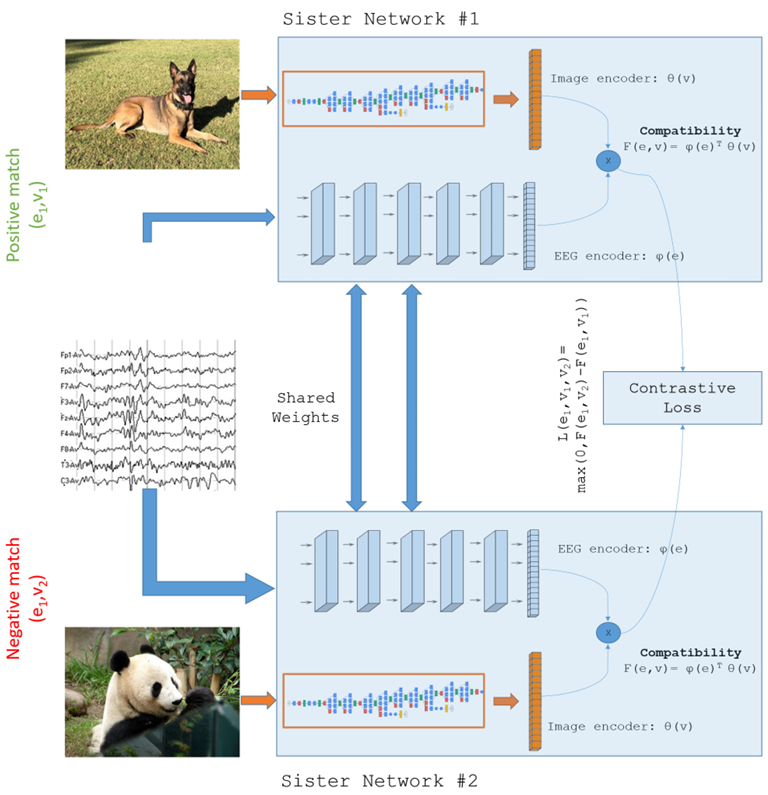
\includegraphics[width=0.6\linewidth]{images/palazzo.png}
    \caption{Siamese network for learning a joint brain-image representation. The idea is to learn a space by maximizing a compatibility function between two embeddings of each input representation. Given a positive match between an image and the related EEG from one subject, and a negative match between the same EEG and a different image, the network is trained to ensure a closer similarity (higher compatibility) between related EEG/image pairs than unrelated ones.}
    \label{fig:palazzo}
\end{figure}

After training, they use the trained EEG and image encoders as feature extractors in the joint embedding space, followed by a softmax layer for image classification, where they classify into 40 classes. They test different configurations of image and EEG encoding in joint embedding, and then quantify each encoder separately as a feature extractor for classification. The results are provided in Table \ref{tab:palazzo}.

\begin{table}[!ht]
    \centering
    \captionsetup{width=.8\linewidth}
    \begin{tabular}{cccccc}
    \hline
    \textbf{Image encoder} & \textbf{EEG} & \textbf{EEG Acc.} & \textbf{Image Acc.} & \textbf{Avg Acc.} \\
    \hline
    Inception-v3 & LSTM & 90.1\% & 93.6\% & 91.9 \\
    \textbf{Inception-v3} & \textbf{GRU} & \textbf{90.4\%} & \textbf{94.7\%} & \textbf{93.0} \\
    \hline
    ResNet-101 & LSTM & 90.7\% & 91.2\% & 91.0 \\
    ResNet-101 & GRU & 92.3\% & 91.5\% & 91.9 \\
    \hline
    DenseNet-161 & LSTM & 92.4\% & 92.3\% & 92.4 \\
    DenseNet-161 & GRU & 93.7\% & 91.8\% & 92.8 \\
    \hline
    AlexNet & LSTM & 85.6\% & 70.1\% & 77.8 \\
    AlexNet & GRU & 77.2\% & 69.9\% & 73.6 \\
    \hline
    \end{tabular}
    \caption{EEG and Image Accuracies refer to accuracy based on EEG encoder and image encoder alone, respectively.}
    \label{tab:palazzo}
\end{table}

In Figure \ref{fig:palazzo_2} is shown how joint embeddings increase performance; merging visual features into EEG features of course boosts EEG classification performance, but is less interesting.\\

\begin{figure}[!ht]
    \centering
    \captionsetup{width=.8\linewidth}
    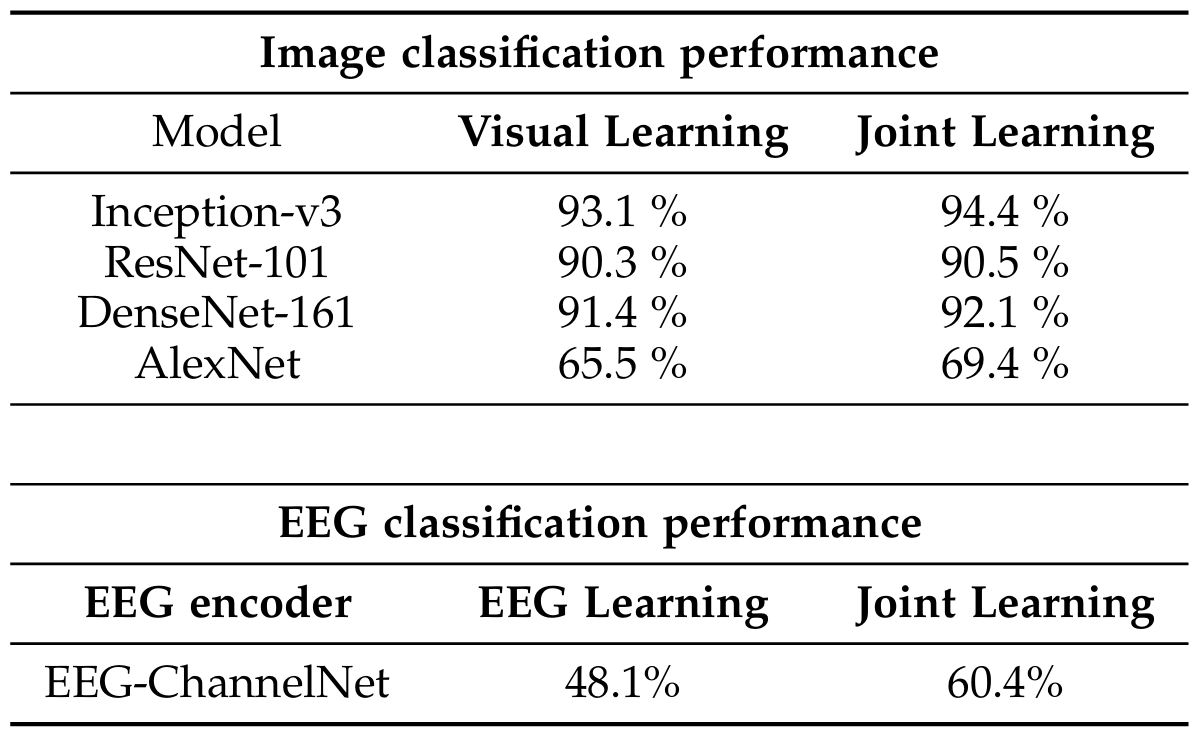
\includegraphics[width=0.5\linewidth]{images/palazzo_2.png}
    \caption{Comparison of image and EEG classification performance when using only one modality (either image or EEG) relative to when the joint neural-visual features are used. For each model, the best performance according to Tab. \ref{tab:palazzo} is reported.}
    \label{fig:palazzo_2}
\end{figure}

Moreover, they \textbf{use the joint embedding for saliency detection} \notet. \textbf{After training for joint embedding}, they employ a masking process. This has to be done after training so that they can trust the compatibility in output of the model. The masking process follows these steps (notice that no learning is involved):
\begin{enumerate}
    \item a mask is applied to a part of the image,
    \item the compatibility between the brain vector (to original image) and the image vector (of the masked image) is computed,
    \item the decrease in match vs. the original compatibility score is computed. 
\end{enumerate}
In other words, the saliency value at pixel $(x, y)$ is obtained by removing the $\sigma \times \sigma$ image region around $(x, y)$ and computing the difference between the original compatibility score and the one after suppressing that patch. This way they understand how much salient an image part is: the higher the decrease in compatibility, the more the saliency. Note that if non-salient parts are removed from the image, the compatibility might increase.

\boxc{\notet Saliency detection}{
Saliency detection is set of algorithms that can process an image to identify which parts of the image are particularly important (outputting a sort of heat map).
These are evaluated by comparing the saliency map generated by the algorithm to the ground truth using either:
\begin{itemize}
    \item Correlation between the two maps;
    \item Normalized Scanpath Saliency (NSS), which computes the mean normalized saliency value at fixated locations (more is better).
\end{itemize}
The ground truth can be obtained using an eye tracker and measuring the ``density" of where people look more.\\

Huang et al. (2015) proposed SALICON, a DNN trained to produce saliency maps. It was created by training an off-the-shelf DNN to predict which parts of the image space were salient. Specifically, a layer is added on top of the last convolutional layer. It contains a single feature, which learns which combinations of feature maps (at that depth) predict pixel saliency (the kernel is $1 \times 1$). Basically, the last layer learns a single kernel that is applied to all pixels. The network is trained with objective functions that maximize the fit to a human saliency map. SALICON can predict saliency at many different image scales by combining information from the original image and its downsampled versions.
}

The experiment consists in participants freely observing the same 2000 images for which EEG data were collected. 
They test competitive saliency-detection algorithms (SALICON and SALNET), in addition to the baseline (effect of masking on simple visual classification, i.e., how much worse a classifier performs when the input image has a masked patch). The results are presented in Fig.~\ref{fig:palazzo_res}.

\begin{figure}[!ht]
    \centering
    \captionsetup{width=.8\linewidth}
    \begin{subfigure}{.49\textwidth}
        \centering
        \captionsetup{width=.8\linewidth}
        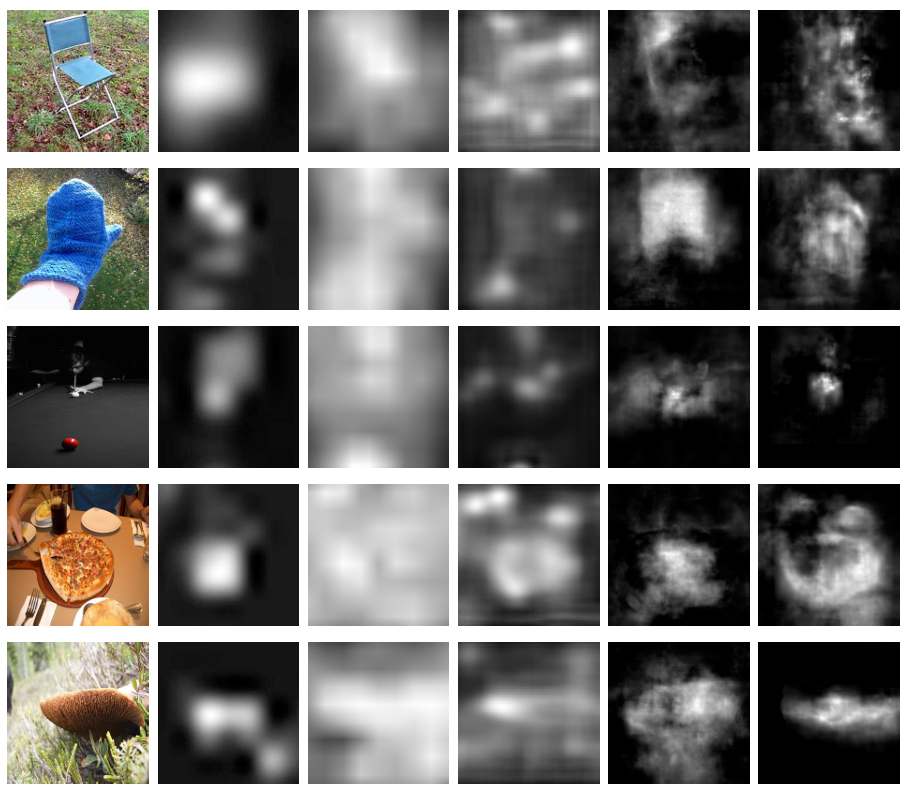
\includegraphics[width=.9\linewidth]{images/palazzo_3.png}
        \caption{Qualitative comparison of generated saliency maps. From left to right: input image, human gaze data (ground truth), SALICON, SalNet, visual classifier–driven detector, and visual/EEG–driven detector (current method).}
        \label{fig:palazzo_3}
    \end{subfigure}
    \begin{subfigure}{.49\textwidth}
        \centering
        \captionsetup{width=.8\linewidth}
        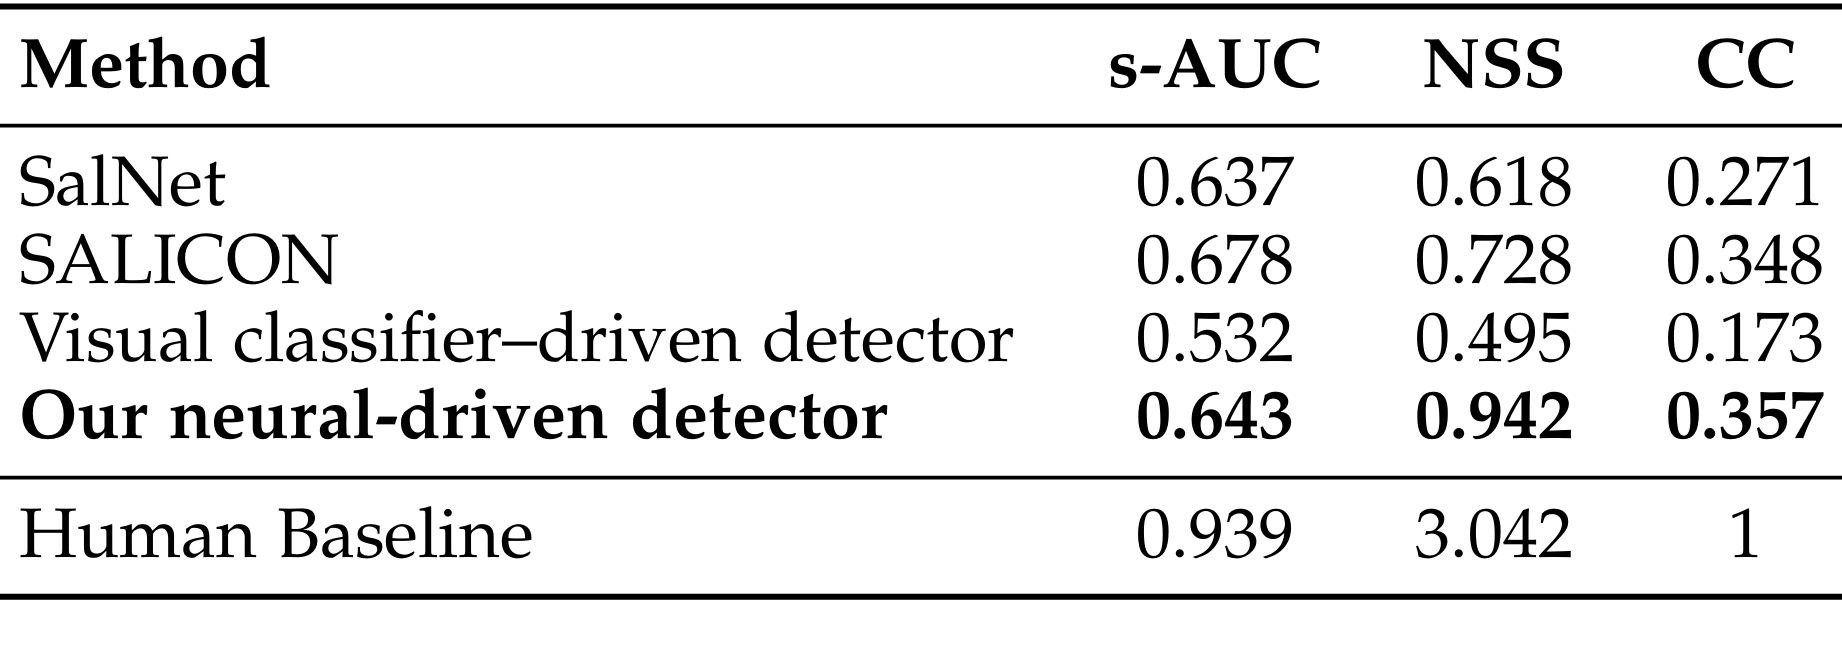
\includegraphics[width=.9\linewidth]{images/palazzo_4.png}
        \caption{ Saliency performance comparison in terms of shuffled area under curve (s-AUC), normalized scanpath saliency (NSS) and correlation coefficient (CC) between the compatibility-driven saliency detector and the baseline models. The human baseline consists in the scores computed using the ground truth maps. Since they adopt a leave-out-one setup, the reported values for their approach are averaged over all the 40 experiments.}
        \label{fig:palazzo_4}
    \end{subfigure}
    \caption{Results of \cite{palazzo2020decoding}.}
    \label{fig:palazzo_res}
\end{figure}

\section[Accommodating human uncertainty]{\textit{Human uncertainty makes classification more robust}\\ Peterson et al. (2019)}
The authors think at accomodating human uncertainty into the network.
We are more interested in modifying the training objective: Should we use a distribution for ground truths, instead of a one-hot encoding?

The main idea is to \textbf{introduce a soft-labelling scheme} that is informed by human uncertainty, and evaluate whether soft labels makes categorization more generalizable to out-of-sample data.

\subsection{Background}

\begin{wrapfigure}[23]{r}{0pt}
  \centering
  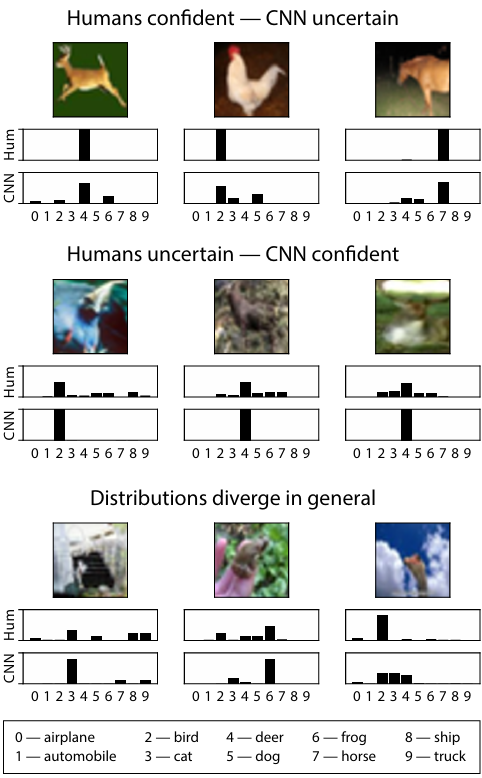
\includegraphics[width=0.35\textwidth]{images/peterson.png}
  \caption{CIFAR10 images for which humans and the best traditionally-trained CNN agree in their top guess, but systematically differ over other choices.}
  \label{fig:peterson}
\end{wrapfigure}
In a classification-learning context, soft labels are ground truth labels for an observation where the mass of the observation is not entirely located at a single correct category.

Many soft labeling schemes have been described:
\begin{itemize}
    \item split mass uniformly among non-target item,
    \item split mass as a function of nearness of an observation to a classification boundary (prevents overfitting),
    \item split mass in relation to types of objects potentially recognized in the scene (categorization and object detection).
\end{itemize}

Human knowledge is inconsistent with the notion of ``hard labels" because in some cases humans are not confident in category assignment, whereas CNNs are. In some cases humans may be not confident, and so will the CNN, but in different ways. \textbf{They propose a method to estimate the soft-label probability distribution from human judgments}. Knowing the human classifications is useful to understand the ``image quality". It is useful for building NNs that reproduce the same sort of vagueness/fuziness.

\subsection{Data and method}
They produce a curated dataset, CIFAR10H: a behavioral dataset consisting of \~500k human categorization decisions over the 10k-image testing subset of CIFAR10 (approximately 50 judgments per image). One of the reason for using  CIFAR10 is that it contains observations close to the category boundaries. They use Amazon Mechanical Turk: on each trial, a person categorizes each image by clicking one of the 10 labels surrounding it as quickly and accurately as possible (but with no time limit). Note: no confidence is obtained for the judgments.\\  

They expect the human image label distribution $p_{hum}(y|x)$ to better reflect the natural distribution over categories given an image, so they use it as an improved estimator for $p(y|x)$, where $y$ is the distribution of activity assigned to all labels for a given image $x$. They then simply use the usual cross-entropy loss to minimize the divergence between the human distribution and the post-softmax activity distribution.

\subsection{Results}
They train multiple architectures using the human labeling data (9k images for training, 1k images for testing). This is simply to show accuracy for the homogenous dataset.
They then apply the learned model (weights) to several other CIFAR10 variants. As generalization measures they evaluate accuracy and cross-entropy loss.\\

As shown in Fig. \ref{fig:peterson_2}, \textbf{generalization improves with human soft labels}. Accuracy is higher and loss is lower using human labels for every individual CNN and dataset.

\begin{figure}[!ht]
    \centering
    \captionsetup{width=.8\linewidth}
    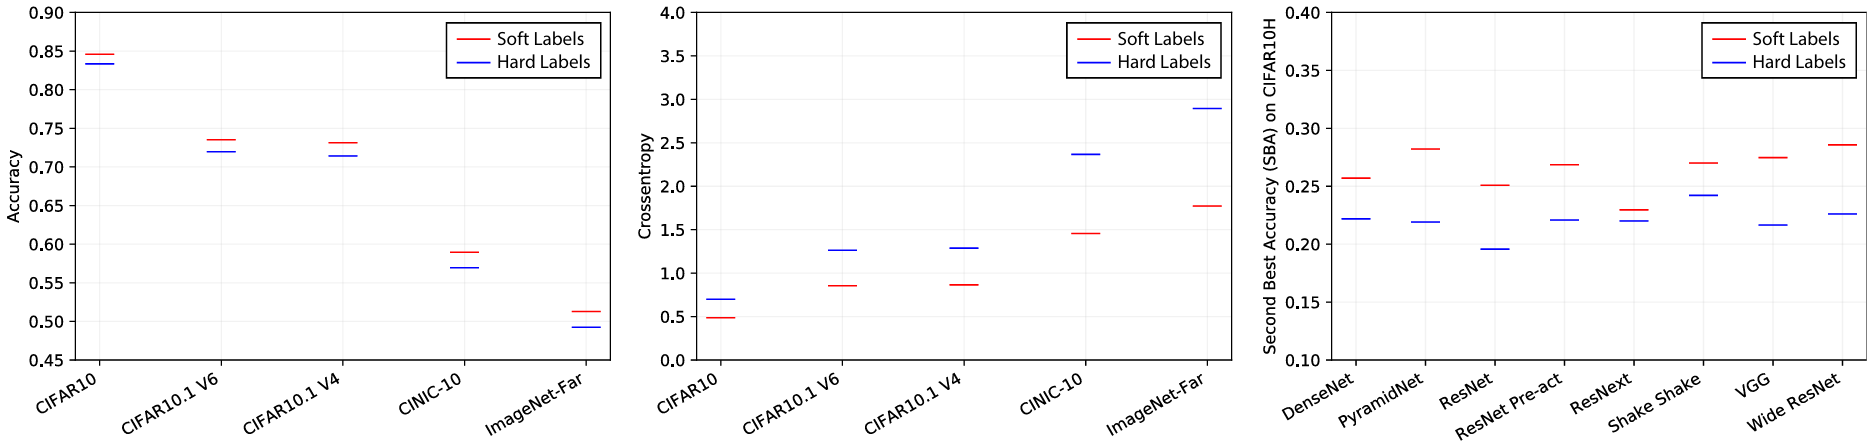
\includegraphics[width=0.9\linewidth]{images/peterson_2.png}
    \caption{Generalization results. Left: accuracy against ground-truth labels, for increasingly out-of-training-sample distributions, averaged across CNNs. Center: cross-entropy against ground-truth labels, averaged across CNNs. Right: Second best accuracy (SBA) for all models using CIFAR10H held out set, averaged across folds.}
    \label{fig:peterson_2}
\end{figure}

\begin{wrapfigure}[14]{r}{0pt}
  \centering
  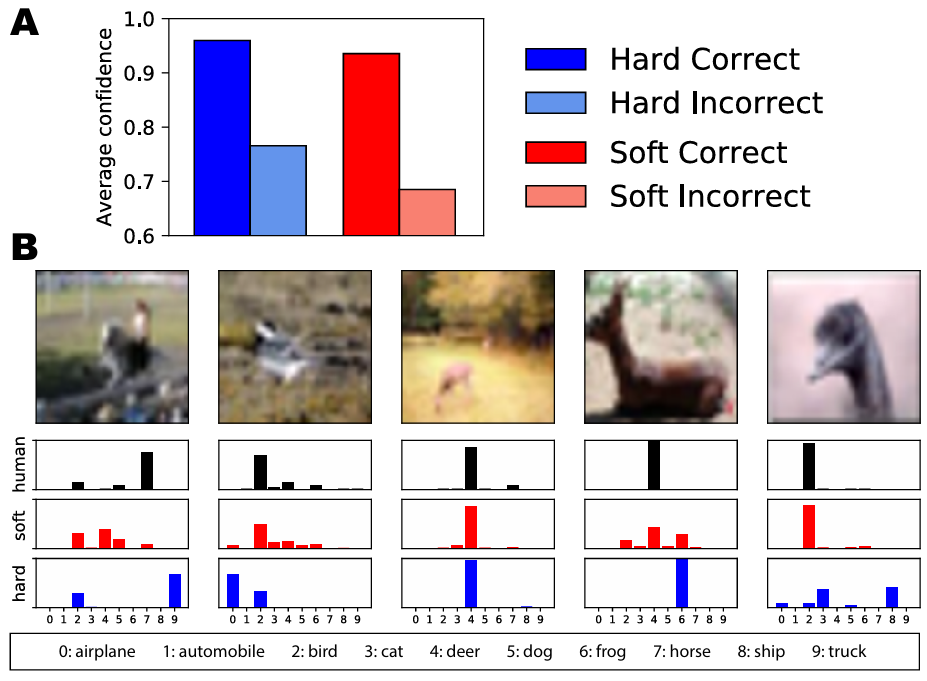
\includegraphics[width=0.35\textwidth]{images/peterson_3.png}
  \caption{\textbf{(A)} Mean confidence for correctly/incorrectly classified examples after hard/soft label training. Soft-label models are far less confident when incorrect than hard-label controls, and only slightly less confident when correct. \textbf{(B)} Soft label training yields predictions that distribute probability mass more like people, with the same top choice.}
  \label{fig:peterson_3}
\end{wrapfigure}

Soft labeling also produces a better calibrated model (\textit{calibration} refers to the relation between confidence of the model and correct/incorrect output). Consider Fig. \ref{fig:peterson_3}: on correct predictions, both hard- and soft-labeling show similar high confidence. Instead, on incorrect predictions, the soft-label training results in significantly lower confidence.\\

They consider several other alternatives to soft labels training. Here are 4:
\begin{itemize}
    \item \textbf{Category soft targets}: approximate category-level confusions by averaging ratings across images within each category. They apply then the same soft label for all images in a category (i.e., all the samples from a category share the same target distribution);
    \item \textbf{Knowledge distillations} an alternative way for simulating confusion (instead of infusing human knowledge): they simulate the confusion by using different models. They take the post-softmax profile of each image from 8 different classification models, averaging.
\end{itemize}

\begin{itemize}
    \item \textbf{Mixup}: a virtual training mechanism that generates merged images (``virtual training examples") and assigns them merged labels.
    \item \textbf{Sampled hard targets}: use human uncertainty in different a way. Based on the human confusion, assign all mass to a single category, but during training ``swap" the labels: for single image train on more than single 1-hot model.
\end{itemize}

Probabilistic soft labels outperform their alternative methods for soft-label construction and also generalize better to new test sets.

\subsection{Discusssion}
Speaking of adversarial attacks, which aim to produce a wrong label for a minimally changed image, the soft-labeling approach provides protection. The accurate behavior here is the maintenance of the original label. Human training produces a network that is much more robust against Fast Gradient Sign Method (FGSM) attacks (one of the easiest ways to create an adversarial image).
Also, when exposed to an adversarial example, the Cross Entropy between the network and the model is lower after being trained with human-trained soft labels. This means that the adversarial example is not shifting the decision as much as it does on a non-soft-label architecture.\\

However, this approach has some potential weaknesses that might be tackled:
\begin{itemize}
    \item the cross-entropy \textbf{loss term for training instance $x$ might be down-weighted if the label for $x$ is determined as not trustworthy or ambiguous}. This does not require setting up a soft label for training, but simply determining which observations are less important than others.
    \item Li et al. (2020) prevent overfitting by \textbf{down-weighting images that are near the decision boundary} of two classes.
    \item In the area of NLP there is a substantial literature on how to incorporate annotator disagreement into models. Fornaciari et al. (2021) find that incorporating soft-label information based on annotator disagreement improves performance on NLP categorization tasks. They add prediction of soft labels as an auxiliary task in Multi-Task Learning: NLP categorization and prediction of soft label distribution (annotators disagreement).
\end{itemize}
